% 来源：OEBPS/Text/Section0001_split_005.xhtml#sigil_toc_id_39

\BookChapter{27}
\section[第27章\q 发大财的时候到了：抗台风的收益和无可匹敌的业绩]{第27章\\ 发大财的时候到了：抗台风的收益和无可匹敌的业绩}

\begin{BookQuote}
如果你什么错误也没犯，却还是输了……你应该要换一种比赛。

\hfill ——尤达大师，《星球大战》
\end{BookQuote}

\subsection{吃了才知道}

我可以很有把握地说，在过去80多年里，我们经历了每种可能的经济季节，还有一些意外，从经济大萧条到大衰退，还有二者之间的那些经济不景气。如果当初就有全天候投资策略，那么在80多年里它表现得如何？我前面说过，我把瑞·达利欧本人亲自给出的全天候投资组合，交给了一个分析师团队，对其进行了广泛的测试，一直回测到1925年！结果震惊了每个人。

我在前面的章节里讲过，过去40多年里全天候投资策略的业绩表现是多么出色。不过，现在我们进一步深入挖掘，我们来看看，在我称之为“现代时期”，即1984—2013年，全天候投资组合的表现如何。结果表明，它跟岩石一样稳健：\footnote{\label{fn:pdf-27-1}这里假定组合每年再平衡。过去的业绩并不能保证未来的业绩。相反，正如我前面说过的，我提供给你的是历史数据，目的是用来讨论和描述基本的投资原则。}

\begin{itemize}
\item 平均年化收益率只是略低于10\%，精确的说是9.72\%（扣费后）。（有一点很重要，这是实际年化业绩，并不是夸大的平均业绩。）
\item 让你这30年里赚钱的年份超过86\%，只有4年是下跌即亏钱的，而且平均亏损只有1.9\%，其中有一年损失只有0.03\%（实质上应该说是盈亏平衡），所以实际上，这30年你只有三年是亏钱的。
\item 你表现最差的那一年是2008年，下跌3.93\%（那一年的标准普尔500指数下跌了37\%）。
\item 书呆子投资者，请注意！标准差只有7.63\%。（这意味着低风险和低波动性。）
\end{itemize}

为什么我们选择从1984年开始的30年？这个时间段标志着401(k)计划的开始，从此每个美国人都成了投资者，股票市场不再只是那些有经验的股市老鸟。年轻人你知道吗，30年前还没有互联网呢！第一部“便携式的”手持电话，即第一部手机，也出现在1984年，摩托罗拉的大哥大手机像块砖头一样大，不仅重，而且贵，接近4000美元。你跟电话公司签约每个月就要交付50美元，打1分钟要花0.5美元。但是你最多只能通话30分钟，因为电池要耗尽了。我这么说就暴露了我这个大叔的年纪了，但我还是非常骄傲，我可是美国第一批用上大哥大的人。

我们不要只说好的方面。我们来看看这个组合的抗压性如何，一定要选在最糟糕的时候——经济冬天。现在金融行业称这种分析为压力测试。

1939—2013年，我称之为历史时期，你看看这些统计数据，会感到太震惊了。（请注意，为了能回测的时间更久，我们会用不同的指数来代表资产配置，我们也不想更换指数，但没办法，因为有些指数在1983年之前并不存在。请看本章末尾所附的测试方法的完整解释。）

% 来源：OEBPS/Text/Section0001_split_005.xhtml → image_720e3dcce7e94eb1bdbddf2e961f5136.jpg
\begin{longtable}{@{}C{\dimexpr 0.50000\linewidth-1.00000\tabcolsep\relax}C{\dimexpr 0.50000\linewidth-1.00000\tabcolsep\relax}@{}}
\caption{标准普尔指数对比全天候投资组合（1939—2013年）}\label{tab:27-1}\\
\toprule\noalign{\vskip 3pt}
{\heiti 标准普尔指数} & {\heiti 全天候投资组合} \\
\midrule
\endfirsthead
\multicolumn{2}{r}{续表}\\[0.6em]
\toprule\noalign{\vskip 3pt}
{\heiti 标准普尔指数} & {\heiti 全天候投资组合} \\
\midrule
\endhead
\bottomrule
\endfoot
\bottomrule
\endlastfoot
75年里标准普尔指数亏损年度18个\footnote{\label{fn:table-表27-1标准普尔指数对比全天候投资组合-1}包括红利再投资} & 同期全天候投资组合亏损年度10个\footnote{\label{fn:table-表27-1标准普尔指数对比全天候投资组合-2}这10个亏损年度中有两年亏损的概率仅为0.03\%（基本上是收支平衡年，因此从实际操作的角度来看，75年里实际上只有8年是亏损的）}（平均略多于10年一次） \\
最大年度亏损43.3\% & 最大年度亏损3.93\% \\
平均年度亏损11.40\% & 平均年度亏损1.63\% \\
\end{longtable}


我们干脆回顾得更久远一些，一直回顾到1927年，这样可以把美国经济历史上发生最大经济萧条的那最糟糕的十年也包括进来。

% 来源：OEBPS/Text/Section0001_split_005.xhtml → image_2dcee32b8b11470b8378d41655b8bec8.jpg
\begin{longtable}{@{}C{\dimexpr 0.50000\linewidth-1.00000\tabcolsep\relax}C{\dimexpr 0.50000\linewidth-1.00000\tabcolsep\relax}@{}}
\caption{标准普尔指数对比全天候投资组合（1928—2013年）}\label{tab:27-2}\\
\toprule\noalign{\vskip 3pt}
{\heiti 标准普尔指数} & {\heiti 全天候投资组合} \\
\midrule
\endfirsthead
\multicolumn{2}{r}{续表}\\[0.6em]
\toprule\noalign{\vskip 3pt}
{\heiti 标准普尔指数} & {\heiti 全天候投资组合} \\
\midrule
\endhead
\bottomrule
\endfoot
\bottomrule
\endlastfoot
87年里标准普尔指数亏损年度24个（占比约27\%）\footnote{\label{fn:table-表27-2标准普尔指数对比全天候投资组合-1}包括红利再投资} & 同期全天候投资组合亏损年度只有14个（这意味着其余73年都是赚钱的） \\
20世纪30年代“大萧条”最严重的时候，1929—1932年标准普尔指数连续4年下跌，累计跌幅64.4\% & 同期全天候投资组合累计亏损20.55\%（优于标准普尔指数59\%） \\
平均年度亏损13.66\% & 平均年度亏损3.65\% \\
\end{longtable}


如果大家说一幢房子是能够抗台风的，要确认这一点的唯一方式就是要经受时间的考验和最强烈台风的考验。下面这张表显示了从1935年以来美国股市的7次暴跌。

% 来源：OEBPS/Text/Section0001_split_005.xhtml → image_673282065b114a2d826aaf55cd26aad5.jpg
\begin{longtable}{@{}C{\dimexpr 0.20000\linewidth-1.33333\tabcolsep\relax}C{\dimexpr 0.40000\linewidth-1.33333\tabcolsep\relax}C{\dimexpr 0.40000\linewidth-1.33333\tabcolsep\relax}@{}}
\caption{自1935年以来最严重的7次暴跌}\label{tab:27-3}\\
\toprule\noalign{\vskip 3pt}
{\heiti 年份} & {\heiti 标注普尔指数（\%）} & {\heiti 全天候投资组合（\%）} \\
\midrule
\endfirsthead
\multicolumn{3}{r}{续表}\\[0.6em]
\toprule\noalign{\vskip 3pt}
{\heiti 年份} & {\heiti 标注普尔指数（\%）} & {\heiti 全天候投资组合（\%）} \\
\midrule
\endhead
\bottomrule
\endfoot
\bottomrule
\multicolumn{3}{@{}p{\linewidth}@{}}{\footnotesize 资料来源：基金投资组合管理工具Jemstep}\\
\endlastfoot
1937 & −35.03\footnote{\label{fn:table-表27-3自1935年以来最严重的7次暴跌-1}包括红利再投资} & −9.00 \\
1941 & −11.59 & −1.69 \\
1973 & −14.69 & 3.67 \\
1974 & −26.47 & −1.16 \\
2001 & −11.89 & −1.91 \\
2002 & −22.10 & 7.87 \\
2008 & −37 & −3.93 \\
\end{longtable}


你一看就会发现，全天候投资策略在这7个冬天里，有两个冬天是上涨的，而且全天候投资策略在另外5个冬天里尽管下跌，但下跌幅度相对要小于美国股市的整体跌幅。我得谈谈这个组合如何对抗股市大势。冬天里，在每个人都冻得发抖、损失严重、内心非常痛苦的时候，这个全天候投资组合让你的损失相对小多了，让你冬天能去滑雪或者玩滑雪板，玩累了还可以享受一杯热巧克力！

再看看最近几年全天候投资组合和市场的业绩表现对比，你会发现领先优势更大了。从2000年1月1日到2014年3月31日，全天候投资组合的涨幅完全超越市场（标准普尔500指数）。在这个时间段里，我们经受了各种各样的瑞·达利欧所说的“重大意外事件”：科技股大崩盘、信贷危机、欧洲债务危机、过去十年多来黄金最大年度跌幅（2013年暴跌28\%）。这个时间段，包括专家所说的股市“失落的十年”，即2000—2009年这十年，标准普尔500指数是平的。你好好看看下面这张图，瑞·达利欧设计的全天候投资组合业绩领先市场的优势有多么巨大：

\begin{figure}[htbp]
\centering
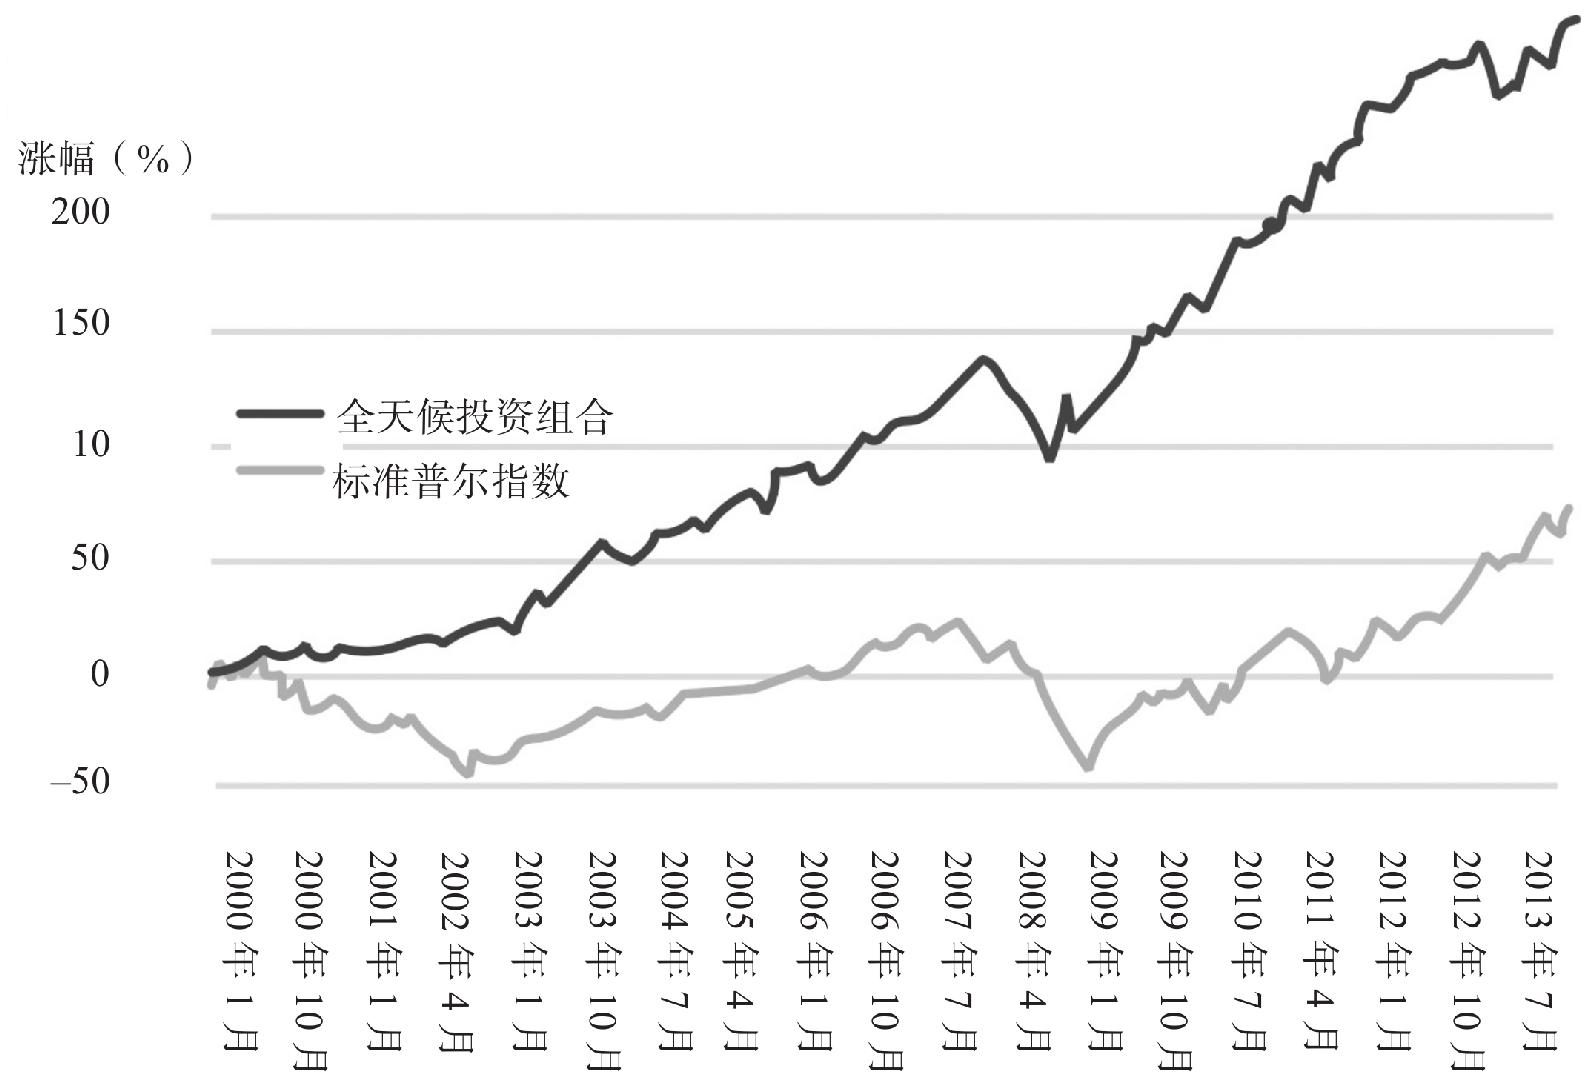
\includegraphics[width=0.96\linewidth,keepaspectratio]{image/27-1.jpg}
\caption{}\label{fig:27-1}
\end{figure}

\subsection{烧个精光}

我们生活在这样一个时代，那些媒体流着口水想要爆料，最想做的轰动新闻就是“让英雄变成狗熊”，把大家都认为是某个阶层里最优秀的代表人物丑化。这既让人看了觉得非常过瘾，又让人心里感到非常悲伤。这些文化人啊，当初就是他们把这些英雄人物捧到高高的完美的偶像塔顶上，可抬得更高只是为了后来摔得更狠。不管是运动员、公司高管，还是基金经理，只要他们盔甲上有一个小小的裂缝，媒体就会大做文章。古罗马人是把有罪的人拉到广场上，朝他们身上掷石头，只不过现在广场换成了媒体和网络，围观的人纷纷吐口水、扔砖头。

我发现一件事让我很吃惊：尽管30年的长期业绩很辉煌，达利欧的全天候投资策略却受到了密集的批评，只是因为2013下跌4\%左右。4\%的跌幅的确很大，但是并不像37\%那么大，就在几年之前，标准普尔500指数就跌了这么多。别忘了，根据历史数据，全天候投资策略也会下跌，但是目标是最小化那些巨幅下跌。我们实话实说，你按照这种全天候投资组合来做投资，可能第一年就会亏损。全天候投资组合的根本目的是稳中求进，而不是用来追求星光璀璨的超高业绩。这是个长期投资策略，追求的是好几十年都尽可能平平稳稳地前进。只看一年的业绩表现来评价这个长期策略，那就大错特错了，你要用好多年的长期业绩整体表现来评价它才公平合理。我写本书的时候是2014年中期，媒体又开始吹捧瑞·达利欧了，因为他全天候投资策略对冲基金在2014年到6月就上涨了11\%。

想想，这些媒体把所有的注意力都只放在一年4\%的亏损上，却提也不提最近5年的业绩表现，2009—2013年全天候投资策略平均每年收益率超过11\%，甚至包括唯一下跌的这个年度，5年业绩还是这么好！但是只是股市上涨的时候，瑞·达利欧的基金反而小幅下跌，结果让他受到了媒体很大的关注，这表明他过去的业绩表现总是高得不可思议、出人意料，现在却跑输市场，这变成了预料之外的事。对于财经媒体来说，评价投资策略只看最近的业绩表现，这就像是评价一个棒球球员有多好，只看他最近一次上场击球表现得有多好。这简直太可笑了。他们竟然根本不顾明摆在那里的事实，瑞·达利欧的对冲基金客户享受到了不可思议的高回报率，一年又一年，一个十年又一个十年，正如《纽约客》杂志2011年一篇报道桥水基金的文章《掌握赚钱机器》所说的那样：

2007年，瑞·达利欧预测到了房地产市场和借贷市场的大繁荣会结束，结局很惨。2007年后期，他警告布什政府，全世界最大的银行很多都处在破产的边沿。2008年，对于很多桥水基金的竞争对手来说，是大灾之年，桥水基金公司的旗舰纯阿尔法基金净值上涨9.5\%，而且是扣费后的业绩。2010年，纯阿尔法基金上涨45\%，创下了大型对冲基金的最高业绩。

关键是有一大堆所谓的专家权威，天天坐在那里，什么也不干，只会说不会做，不管你用什么策略，他们都会把你批评得一无是处。对于这种人，我最喜欢用戴维·巴贝尔博士说的那句话：“让他们批评去吧，我们去睡觉。”

\subsection{好问题}

谈到全天候投资策略，博客上提得次数最多的问题是：利率上升会发生什么样的情况？政府债券会不会下跌，导致整个组合发生亏损。因为这个组合配置在债券上的资产比例很大呢？

这个问题提得很好，值得讨论，但是也不过是一个人坐在场外指手画脚罢了。第一，你要记住，把一部分资产配置在债券上，并不是只赌债券。这个投资组合把你的风险分散在四种可能遇到的不同经济季节上。

瑞·达利欧向我们展示了，关键不是做好计划应对某一个具体的季节，或者假装知道下一个到来的会是什么季节。记住，意外肯定会发生，会让大多数人猝不及防。

事实上，很多人一直努力地在劝诱大家信奉他，预测下一个季节会是什么，他们呼吁利率要快速上涨。毕竟金融危机之后，我们现在的利率水平是有史以来最低的，但是麦克·欧希金斯在她的著作《战胜道琼斯指数》里写道，人们也许要等待相当长的时间，才能盼到利率大幅上涨，因为美联储历史上曾经就这么做过，长期压制利率在很低的水平，以保持借贷成本处于低位：“对于绝大多数投资者来说，他们相信，接下来的一年（2014），利率不可避免地会走高，记住，美联储曾经长期把利率水平压制在3\%以下，连续22年，从1934年一直压制到1956年。”

2008年以来，美联储一直保持低利率，所以谁也不知道低利率还会保持多久。没有人能告诉你一个确定的答案。2014年早期，每个人都预期利率会上升，结果利率再次下降，引发美国债券价格大涨。（记住，利率下降，债券价格会上升。）

全天候投资策略在利率上升的市场会表现如何呢？

有一个回顾性的练习：回看历史，在一个利率像热气球一样快速上升的经济季节里，全天候投资组合会发生什么样的情况？上一次利率下跌好几十年之后，1970—1979年出现了快速通货膨胀。尽管利率像火箭一样飙升，全天候投资组合在1970—1979这十年间只有1年是亏损的，这十年取得的年化收益率是9.68\%。其中包括1973年和1974年两个年度背靠背下跌，标准普尔指数先是下跌14.31\%，然后又下跌25.90\%，累计下跌40.21\%。

所以就让电视上看起来脑袋很大好像智慧也很大的那些专家权威去高谈阔论吧。他们想说服我们相信他们知道下一个到来的会是什么季节。但是我们一定要扎实地准备好应对所有四种季节，还有前面肯定会碰到的各种各样的重大意外事件。

\subsection{让我们面对现实吧}

全天候投资组合最后一个也是至关重要的优势是，它有很多人性化的成分。很多批评家会指出，如果你有勇气承担更多的风险，你就能够战胜这种全天候投资策略。他们说的也许是对的，但是全天候投资组合的关键是减少波动性，即风险性，同时继续把收益最大化。

如果你还年轻，投资期限还很长，或者尽管你年纪不小了，但是你愿意承担更多的风险，在这两种情况下，你当然可以充分利用全天候投资策略的整体资产配置方案，但是你可以做一个小小的调整，股票增加一些，债券减少一些，以产生更高的收益率。但是，牢记在心，这样改变配置会增加风险，即波动性，其实你这样做是更多地下注在一种季节上（在这个季节里你希望股票会上涨）。过去，你要是这样多配股票、少配债券，效果会非常好。你访问一下堡垒投资理财公司的网站，就会看到，长期来看，配置更多的股票，会让投资组合产生的收益率更高，但是同时在某些年份也发生更大的下跌。但是，正是这个地方很有意思，简直不可思议。和标准的60∶40平衡投资组合（60\%的资产购买标准普尔500指数和40\%的资产购买伯克利债券指数）相比，全天候投资策略提高股票配置比例之后，仍能轻松跑赢。你使用传统的60∶40投资组合，就不得不接受高出80\%的风险（标准差），不过业绩仍然稍逊于提高股票资产配置比例之后的全天候投资组合。

但是我们对自己一定要诚实，我们的承受力要比我们装给别人看的要弱得多。研究机构刀疤（Dalbar）揭示出我们对风险的真实消化能力究竟有多大。从1993年12月21日到2013年12月31日这20年，标准普尔500指数年化收益率为9.2\%，但是公募基金投资者的平均年化收益率只是2.5\%多一点儿而已，勉强能战胜通货膨胀。\footnote{\label{fn:pdf-27-2}数据来源：Richard Bernstein Advisors LLC, Bloomberg, MSCI, Standard \& Poor’s, Russell, HFRI, BofA Merrill Lynch, Dalbar, FHFA, FRB, FTSE.所有收益均以美元计算。}要是事先知道是这样，你还不如去投资3个月期限的美国短期国债，接近于现金等价物，收益率反而更高，还能避免股市下跌让你晚上翻来覆去地睡不着觉。

\subsection{为什么普通投资者真正赚到手的钱这么少？}

Dalbar总裁路易斯·哈维说：“投资者把他们的钱在市场上进进出出，时机却不对。他们要么过度兴奋，要么过度害怕，他们是自己害了自己。”

还有一个更令人感到震惊的案例，那是全球最大公募基金公司之一富达基金做的一项研究。富达投资集团研究了自己的旗舰产品麦哲伦基金的业绩表现。起初管理麦哲伦基金的基金经理是彼得·林奇\footnote{\label{fn:pdf-27-3}我很荣幸访问过彼得·林奇，请他讲述他的核心投资原则，正好是在他创造最伟大的投资连续战胜股市13年的投资奇迹期间，他在我的财富大师训练营上发表过演讲，那是在1990年早期。}，他可是投资界的传奇巨星，1977—1990年的年化收益率为29\%，高得太惊人了。但是富达基金公司发现，那些买过麦哲伦基金的投资人，平均而言，实际上都是亏钱的！这怎么可能呢？富达投资集团的研究表明，当基金净值下跌的时候，投资者就会赎回基金兑现走人，因为他们害怕继续下跌会亏得更多。当基金净值上涨的时候，他们就会纷纷跑回来了，高位买入，而且越涨越买，像个非常大方的投资者。

事实真相是这样的：很多投资者根本承受不了再来一个2008年那样的股市暴跌，没有人做到不卖出手上的股票或基金。这就是人性。所以，当人们谈论更好的业绩时，对于大多数人来说，他们谈的是一个虚构的投资者——这个人有钢铁般的神经，还有一大抽屉抗胃酸药。有个很合适的例子，我最近在市场观察网站上浏览时偶然看到一篇赫伯特写的文章。马克追踪了投资者订阅那些时事通讯的业绩表现，这些通讯告诉投资者精确的买入和卖出的时间点，以精准把握市场时机。表现最好的时事通讯，过去20年的年化收益率高达16.3\%。这是相当杰出的业绩表现，至少可以这么说。但是有业绩表现特别好的年份，也就有业绩表现特别差的年份。正如马克·赫伯特所解释的那样：“那种很高的业绩表现会让你反胃，2000—2003年这三个市场循环里，它的业绩表现属于同类表现中最差的。例如，2007—2009年这波大熊市里，它提供的模板投资组合下跌接近2/3。”2/3？那就是66\%！你能想象吗，你投资10万美元，现在只剩下3.3万美元？要是你投资了100万美元，现在就只剩下33万美元，你心里能够承受得住这么大的亏损，继续坚定持有下去吗？

马克·赫伯特问这份时事通讯的出版人，投资者是不是真的会继续坚定地持有你推荐的投资组合，即使是在这样业绩过山车般大起大落的时候，他只是轻描淡写地在邮件里回答说，第一次从广泛分散投资组合中跳出来的投资，并不适合用他的这种投资策略，如果用他的这种策略，会有一些担心。”

我会觉得66\%的下跌可不只是让人有“一些担心”而已，他的说法听起来好像是，我们这些肉身凡人容易过度反应，就好像我一看到汽车仪表盘上检查引擎的警示灯亮起，就会从一辆正在奔驰的汽车上跳出来一样。记住，66\%的亏损之后，要求你必须再获得接近200\%的收益率，才能赎回你的本金，实现盈亏平衡——只是为了弥补你亏掉的那些养老金，可能就需要花费你一辈子攒的钱！

% 来源：OEBPS/Text/Section0001_split_005.xhtml → image_587e465408ca43a284761d84fa20ac43.jpg
\begin{longtable}{@{}C{\dimexpr 0.50000\linewidth-1.00000\tabcolsep\relax}C{\dimexpr 0.50000\linewidth-1.00000\tabcolsep\relax}@{}}
\caption{如果亏损，你以后回本需要赚的钱}\label{tab:27-4}\\
\toprule\noalign{\vskip 3pt}
{\heiti 如果你亏损} & {\heiti 回本需要赚的钱} \\
\midrule
\endfirsthead
\multicolumn{2}{r}{续表}\\[0.6em]
\toprule\noalign{\vskip 3pt}
{\heiti 如果你亏损} & {\heiti 回本需要赚的钱} \\
\midrule
\endhead
\bottomrule
\endfoot
\bottomrule
\endlastfoot
5\% & 5\% \\
10\% & 11\% \\
15\% & 18\% \\
20\% & 25\% \\
25\% & 33\% \\
30\% & 43\% \\
35\% & 54\% \\
40\% & 67\% \\
45\% & 82\% \\
50\% & 100\% \\
75\% & 300\% \\
90\% & 900\% \\
\end{longtable}


无一例外，我为写作本书采访的理财大师都执迷于不要亏本。他们明白，只要亏本了，以后你必定要赚得更多才能回本——重新回到盈亏平衡，折腾来折腾去，一分钱也没有赚到。

真相是，如果我们对自己诚实的话，我们都会对自己的投资做出情绪化的决策。我们都是有情绪的动物，没有情绪那就不是人类了，甚至是这个世界上最优秀的交易者也在跟内心的恐惧做斗争。这种全天候投资组合能够保护你避免任何潜在经济环境的伤害，也会避免给自己造成伤害！全天候投资组合提供了“情绪上的支架”，让你避免做出糟糕的决策。如果在过去75年里，即使在股市跌得最糟糕的年份里，你也只不过是亏了3.93\%，你怎么会吓得人都崩溃了，一下子全部抛出呢？2008年，整个世界就像发生了火灾，一切都烧了个精光，但是你的全天候投资组合只下跌了3.93\%，而其他人的投资组合很多跌了一半，甚至更多，人好像要崩溃了。相比之下，你会觉得你的内心是多么的平和宁静啊。

你已经有这样让你安度惊涛骇浪却如履平地的投资组合了！全天候投资组合，带有详细配料的比例，它来自投资界的大神级“大厨”瑞·达利欧。要做他的基金客户，得到他的投资建议，你至少要有50亿美元资产。现在你不用等到自己有50亿美元的财富，就可以得到他的投资组合建议，你付出的代价只是购买本书的钱。他自己管理对冲基金，实际使用的就是全天候投资组合，为了便于个人投资者使用，他做了一些简化，去掉了融资杠杆，也采取了更加被动的投资方式，即利用指数基金去做投资。（被动投资就是努力跟随市场，而不是努力战胜市场，成为最好的选股者或者最好的预测者，努力准确地预测接下来会是什么样的投资季节。）你完全可以自己动手，按照瑞·达利欧推荐的这个全天候投资组合去做配置，但是如果你想这样做的话，我要提醒你注意以下几点：

\begin{itemize}
\item 你选择的低成本指数基金，或者交易所交易基金会改变业绩。至关重要的是，要给每个资产类型，找到最有效和成本效率最高的代表性指数基金产品，来配置每个百分比的资产。
\item 组合需要持续监控，每年进行再平衡。
\item 组合有时税收率不高，就是说同样的收益，交的税太多。重要的是运用你的退休金账户或者其他有税收效率的投资结构，来适当地最大化税收效率。你可以用低成本可变年金，就像美国教师退休基金会或者先锋公司提供的可变年金产品。（不管怎么样，只有这两个产品似乎是让那些投资专家一致赞同物有所值的产品。）
\end{itemize}

\subsection{全天候+终身收入}

堡垒理财网的团队，最近将全天候投资组合作为他们众多客户的投资选择之一。有些读者想自己动手实施这个投资组合，而另外一些投资者可能更愿意找专业人士帮忙，找个受托人投资顾问，就像堡垒理财网。选择哪种方式都行，只要对你最有利。关键是抓紧采取行动。

\subsection{采取大行动}

该你做出行动了。如果你有更好的策略，事实证明有效，可以让下行风险损失最小化而让上行收益最大化，也许你应该出来创办自己管理的对冲基金。现在，该有的信息都有了，相当于全副武装，你完全可以自己动手，像瑞·达利欧建议的那样搞一个全天候投资组合了，或者如果你愿意的话，也可以找一个受托人，帮助你构建和监控一个全天候投资组合，作为一个综合性投资理财计划的其中一部分。

如果你想创建自己的个人计划，最多只用5分钟，请登录堡垒网看看你现在的投资组合策略的业绩表现，能不能比得上其他渠道提供的一系列投资策略，包括我们这里讲的全天候投资策略。

\subsection{让你的经理人试驾}

堡垒理财网赠送的分析能让你“看到引擎盖下”，看到你在别的地方根本看不到的真相：你真正支付的费用是多少，你现在的投资真正的业绩表现怎么样。堡垒理财网的分析还会特别强调指出，你现在承受的风险有多大，过去15年你真正的业绩是多少。在这15年里我们经历了两次接近腰斩的暴跌（2000年2月和2008年9月）。

如果你选择采取行动，你可以把你的账户在线转到堡垒理财网，然后今天就开始这一套分析。如果你不愿意转移账户，也没关系，你依然可以免费获得你需要的全部信息。

\subsection{我的401(k)账户怎么办？}

全天候投资策略也可以被运用到你现有的401(k)计划之中，只要你的计划里有合适的基金可供选择，能代表瑞·达利欧推荐投资的资产类型就行。你可以自己操作，也可以请投资顾问来帮助你操作。如果你使用堡垒理财网，它会自动把你的401(k)账户连接到你的整体计划，确保401(k)账户的投资组合设置正确。另外，还有美国最好401(k)，也可以提供给你全天候投资策略。

\subsection{收入就是结果}

前面两章我们已经覆盖了很大的金融投资领域。但是到现在，我想你能够看明白其中的原因了。现在掌握在你手里的是一个投资计划，它有傲人的历史业绩记录，无与伦比！你可以自己动手交易，构建出这样一个投资组合，只用几分钟就行，从此你再也不用生活在忧虑之中，天天担心市场的涨跌。没有人知道未来会怎么样，但是历史会告诉你，你这样做，无论以后是什么样的经济季节，什么样的经济情况，你都做好了充分的准备，都能得到保护。

那么现在让我们回到我们原来说过的投资比喻：个人的珠穆朗玛峰。使用全天候投资策略，你就能有最好的概率步伐平稳，持续稳定地前进，顺利地攀爬到顶峰。是的，路上会出现意外，但是这个投资组合会更加健康、更加强大，经过长期的时间，你就会取得成功。现在，请你记住，只要你已经持续不断地提升你的投资价值，达到关键规模，你就会有足够的财富实现财务自由，你需要最终把你的养老金（就是这些投资）转换成有保障的收入流——你自己的终身收入计划。有了它，再也不用非得靠工作来赚钱维持生活了。这正是最终能够给我们带来财务自由的源泉。让我们翻开下一页，学习为什么“全天候投资组合+终身收入=真正的财务自由”。让我们来学习如何创造一份终身收入。

\subsection{瑞·达利欧如此非凡的投资业绩是怎样做到的？}

瑞·达利欧是如何做到持续产生如此非凡的投资收益的呢？他已经搞懂，这个巨大的经济体是一个巨大的机器，所有事物都通过某种方式连接在一起。有时连接很明显，但很多时候连接并不明显。瑞·达利欧可以看透整个经济机器，知道部分可预测的模式，他能够从中获利。他对经济体系的研究成果被浓缩成了一段30分钟的视频，非常精彩，按照我个人的观点，每一个投资人都应该看一看！瑞·达利欧，决定制作这个视频，不单是为了影响社会，而且是为了帮助大家进行经济学扫盲，让你从此不再觉得经济学高深莫测，让我们了解这个世界运转的经济真相。花上30分钟，好好看看瑞·达利欧制作的这段视频经济课，你会一辈子都庆幸自己做了这件事。

\subsection{我们是如何计算投资业绩的？}

我们在这里讲了很多次全天候投资组合的历史模拟投资业绩，为了保证这些业绩数据的准确性和可信度，我们组建了一个分析师团队测试这个投资组合，使用的都是低成本且广泛分散的指数基金。为什么这对你来说很重要呢？运用真实的指数基金业绩数据，而不是从理论上构造出一个指数数据，这样的数据只是由理论推导出来的，并不是真实指数基金的真实业绩。本章列出的所有业绩，都完全包括基金每年的费用和基金追踪指数的误差。这样做对你有好处，可以展示给你看全天候投资组合的真实历史业绩（而不只是在纸面上用来回测的理论业绩）。这样做可以保证回测这个全天候投资组合使用的基金和数据，一般人现在都能够得到，而不只是那些有好几十亿资产管理规模的华尔街金融机构才能得到。不过，有时候，我们回测时还是不能运用真实的指数基金数据，因为那个时候，指数基金根本不存在，我们分析师团队对每个资产类型都用分散范围很大的指数涨跌幅数据，然后再按照基金费用调整为扣费后的业绩，来模拟指数基金业绩。注意，他们在计算时运用了每年一次的再平衡，假设所有这些投资都是持有在一个免税账户里的，没有交易成本。最后，我要感谢克里夫·斯科曼、西蒙·罗伊，还有整个Jemstep团队做出的深入分析，还有堡垒财富管理公司的阿杰伊·古普塔在这个项目中的合作。（过去的业绩并不能保证未来的业绩。）
